% start the document

% specify the document layout and font size
\documentclass[preprint,12pt]{elsarticle}
% \documentclass[final,twocolumn,12pt]{elsarticle}
% \usepackage[margin=1.5cm,includefoot]{geometry}
\usepackage{setspace}

% uploading packages
\usepackage{graphicx}
\usepackage{amssymb}
\usepackage{textcomp} % https://latex.org/forum/viewtopic.php?f=4&t=3364#p13124, https://tex.stackexchange.com/questions/165115
\usepackage{gensymb}
\usepackage{lineno}
\usepackage{mathtools}
\usepackage[title]{appendix}
\usepackage{pgfmath}
\newcommand{\calcnum}[1]{%
    \pgfmathparse{#1}%
    \num[round-mode=places,round-precision=1]{\pgfmathresult}%
}
\usepackage[separate-uncertainty=true]{siunitx} % \usepackage{xr-hyper} %needs to  be before hyperref
\usepackage{xurl} %needs to be before hyperref
\usepackage[colorlinks]{hyperref}
\hypersetup{breaklinks=true} % set automatically by hyperref?
% \PassOptionsToPackage{hyphens}{url}\usepackage{hyperref} %allow URLs to break across lines
\usepackage[nameinlink,capitalise]{cleveref} %needs to appear after hyperref, https://tex.stackexchange.com/questions/396728/my-equations-referencing-not-working
\Crefname{figure}{Figure}{Figures} %needs to appear after hyperref and cleveref
\crefname{appsec}{Appendix}{Appendices}
\newcommand\crefrangeconjunction{--} % modify the reference style
\usepackage{mathrsfs}
\usepackage{enumitem}
\usepackage{tabulary}
\usepackage{caption}
\usepackage{subcaption}
\usepackage{multirow}
\usepackage{makecell} % https://tex.stackexchange.com/questions/2441/how-to-add-a-forced-line-break-inside-a-table-cell
\newcommand{\NA}{---} % holds an m-dash
\graphicspath{{figures/}} %Setting the graphicspath
% ---------to deal with the double quotes----------- 
\usepackage [english]{babel}
\usepackage [autostyle, english = american]{csquotes}
\MakeOuterQuote{"}
\usepackage{listings}[breakatwhitespace=true,escapechar=\%]
\usepackage{matlab-prettifier}
\newcommand{\matlab}[1]{\mbox{\lstinline[style=Matlab-editor]{#1}}}
%alternatively can use `` '' format for double quotes
\usepackage{booktabs}
\setlength{\abovetopsep}{1ex}
\usepackage[shortcuts,abbreviations]{glossaries-extra}
\newcommand*{\TCac}[1]{\ecapitalisewords{\glsentrylong{#1}}}
% remove the "Preprint submitted to Elsevier" footer on the first page
\makeatletter
\def\ps@pprintTitle{%
   \let\@oddhead\@empty
   \let\@evenhead\@empty
   \def\@oddfoot{\reset@font\hfil\thepage\hfil}
   \let\@evenfoot\@oddfoot
}
\makeatother

% Cross referencing with the xr package in Overleaf (https://www.overleaf.com/learn/how-to/Cross_referencing_with_the_xr_package_in_Overleaf)
\makeatletter
\newcommand*{\addFileDependency}[1]{% argument=file name and extension
  \typeout{(#1)}
  \@addtofilelist{#1}
  \IfFileExists{#1}{}{\typeout{No file #1.}}
}
\makeatother
\newcommand*{\myexternaldocument}[1]{%
    \externaldocument{#1}%
    \addFileDependency{#1.tex}%
    \addFileDependency{#1.aux}%
}

\usepackage{nameref,zref-xr}
\zxrsetup{toltxlabel}
%https://tex.stackexchange.com/questions/77774/undefined-control-sequence-when-cross-referencing-with-xr-hyper
% \myexternaldocument{supp}

\biboptions{sort&compress}
\interfootnotelinepenalty=10000 %prevent footnotes from getting split across columns/pages 
%\patchcmd{\emailauthor}{(#2)}{(S.G. Baird).}{}{} %Removes/Abbreviates corresponding author name after Email address so that the footnote doesn't take up 2 lines.
% Double Spacing
% \doublespacing
\usepackage[margin=1.5cm,includefoot]{geometry}
\usepackage{auto-paper}
% \PassOptionsToPackage{refcheck}{auto-paper} %comment this out before submission

\zexternaldocument*{main-frankenstein-2} %try deleting log files if producing an error, see https://tex.stackexchange.com/questions/131709/unclean-aux-file-causes-file-ended-while-scanning-use-of-newlbel-error-wh
% Concatenate the different "values" .tex files
%RMSE values
% \newcommand{\baryrmse}{0.0242}
% \newcommand{\gprrmse}{0.0220}
% \newcommand{\idwrmse}{0.0345}
% \newcommand{\nnrmse}{0.0448}
% \newcommand{\avgrmse}{0.1302}
% %paper-data6
% \newcommand{\baryrmse}{0.0238}
% \newcommand{\gprrmse}{0.0218}
% \newcommand{\idwrmse}{0.0356}
% \newcommand{\nnrmse}{0.0445}
% \newcommand{\avgrmse}{0.1283}
%\newcommand{\gprrmsePercReduction}{83}
% paper-data9
\newcommand{\baryrmse}{0.0239}
\newcommand{\gprrmse}{0.0217}
\newcommand{\idwrmse}{0.0343}
\newcommand{\nnrmse}{0.0448}
\newcommand{\avgrmse}{0.1284}
\newcommand{\gprrmsePercReduction}{83.1}

%MAE values
% \newcommand{\barymae}{0.0145}
% \newcommand{\gprmae}{0.0145}
% \newcommand{\idwmae}{0.0223}
% \newcommand{\nnmae}{0.0307}
% \newcommand{\avgmae}{0.0965}
% %paper-data6
% \newcommand{\barymae}{0.0145}
% \newcommand{\gprmae}{0.0145}
% \newcommand{\idwmae}{0.0225}
% \newcommand{\nnmae}{0.0307}
% \newcommand{\avgmae}{0.0955}
%paper-data9
\newcommand{\barymae}{0.0145}
\newcommand{\gprmae}{0.0145}
\newcommand{\idwmae}{0.0223}
\newcommand{\nnmae}{0.0308}
\newcommand{\avgmae}{0.0959}

%\newcommand{\nnomega}{2.8709 \pm 0.69112}
\newcommand{\nnomega}{2.8702 \pm 0.69117}

\newcommand{\symtime}{76}

\newcommand{\nigprbrkrmse}{0.1471}

%Supplementary
\newcommand{\thr}{\SI{1.1}{\joule\per\square\meter}}
\newcommand{\sigthr}{\SI{1.1}{\joule\per\square\meter}}
\newcommand{\thrtwo}{\SI{1.2}{\joule\per\square\meter}}


%% main-frankenstein-2
\newcommand{\minsymdist}{$\sim$\SI{64.0}{\tobydeg}}
\newcommand{\percExplained}{$\sim$\SI{99.6}{\percent}}
\newcommand{\percFiveVsOne}{$\sim$\SI{70}{\percent}}
\newcommand{\dimOne}{$\sim$\SI{65}{\tobydeg}}

% figure info, etc. that can dynamically change (color of points, etc.)
\newcommand{\startpt}{red points}
\newcommand{\singlept}{magenta points}
\newcommand{\sympt}{dark blue points}
\newcommand{\singlesympt}{dark blue point}
\newcommand{\refpt}{white circle}
\newcommand{\vbordercolor}{black}
\newcommand{\vcellcolor}{light blue}
\newcommand{\inpt}{input}
\newcommand{\outpt}{prediction}
% \newcommand{\inptvar}{ninputpts}
% \newcommand{\distfn}{GBdist4}
\newcommand{\vfzorepo}{\gls{vfz} repository}
\newcommand{\mytitleone}{Five Degree-of-Freedom Property Interpolation of Arbitrary Grain Boundaries via \glsentrytitlecase{vfz}{long} Framework}
% \newcommand{\mytitletwo}{Properties of a \glsentrytitlecase{5dof}{long} \glsentrytitlecase{fz}{long} defined via \glsentrytitlecase{vfz}{long} Framework}
\newcommand{\mytitletwo}{$O_h$ \glsentrytitlecase{5dof}{long} \glsentrytitlecase{fz}{long} Properties via \glsentrytitlecase{vfz}{long} Framework}
\makeglossaries
\GlsXtrEnableEntryCounting{abbreviation}{3}
% \glssetcategoryattribute{abbreviation}{indexonlyfirst}{true}
\glssetcategoryattribute{abbreviation}{nohyper}{true}

% \setabbreviationstyle[abbreviation]{long-short}

% \glsenableentrycount
% \glssetcategoryattribute{abbreviation}{entrycount}{2}

\newabbreviation[longplural=five degrees of freedom]{5dof}{5DOF}{five degree-of-freedom}
\newabbreviation[longplural=three degrees of freedom]{3dof}{3DOF}{three degree-of-freedom}
\newabbreviation[longplural=degrees of freedom]{dof}{DOF}{degree of freedom}
\newabbreviation{ebsd}{EBSD}{electron backscatter diffraction}
\newabbreviation[longplural={grain boundaries}]{gb}{GB}{grain boundary}
\newabbreviation{fcc}{FCC}{face-centered cubic}
\newabbreviation{sem}{SEM}{scanning electron microscope}
\newabbreviation{fea}{FEA}{finite element analysis}
\newabbreviation{bcs}{BCs}{boundary conditions}
\newabbreviation[longplural={triple junctions}]{tj}{TJ}{triple junction}
\newabbreviation{gpr}{GPR}{Gaussian process regression}
\newabbreviation{gprm}{GPRM}{Gaussian process regression mixture}
\newabbreviation{ann}{ANN}{artificial neural network}
\newabbreviation{nn}{NN}{nearest neighbor}
\newabbreviation{rmse}{RMSE}{root mean square error}
\newabbreviation{mae}{MAE}{mean absolute error}
\newabbreviation{brk}{BRK}{Bulatov Reed Kumar}
\newabbreviation{gbed}{GBED}{grain boundary energy distribution}
\newabbreviation{gbcd}{GBCD}{grain boundary character distribution}
\newabbreviation{mfz}{MFZ}{misorientation fundamental zone}
\newabbreviation{bp}{BP}{boundary plane}
\newabbreviation{bpfz}{BPFZ}{boundary plane fundamental zone}
\newabbreviation{knn}{kNN}{k-nearest neighbor}
\newabbreviation{gbe}{GBE}{grain boundary energy}
\newabbreviation{gbo}{GBO}{grain boundary octonion}
\newabbreviation{nbo}{NBO}{no-boundary octonion}
\newabbreviation{oslerp}{oSLERP}{octonion Spherical Linear Interpolation}
\newabbreviation{loocv}{LOOCV}{leave-one-out cross validation}
\newabbreviation{kfcv}{kFCV}{k-fold cross validation}
\newabbreviation{seo}{SEO}{symmetrically equivalent octonion}
\newabbreviation{fex}{FEX}{file exchange}
\newabbreviation{idw}{IDW}{inverse-distance weighting}
\newabbreviation{fic}{FIC}{fully independent conditional}
\newabbreviation{svd}{SVD}{singular value decomposition}
\newabbreviation{gbc}{GBC}{grain boundary character}
\newabbreviation{fz}{FZ}{fundamental zone}
% \newabbreviation{pfz}{pFZ}{pseudo fundamental zone} % pfz replaced by vfz
% \newabbreviation{cmo}{CMO}{closed-mesh octonion} % cmo replaced by vfzo
\newabbreviation{vfz}{VFZ}{Voronoi fundamental zone}
\newabbreviation{vfzgbo}{VFZ-GBO}{Voronoi fundamental zone grain boundary octonion}
\newabbreviation{lobpcg}{LOBPCG}{locally optimal block preconditioned conjugate gradient}
\newabbreviation{lkr}{LKR}{Laplacian kernel regression}
\newabbreviation{ms}{MS}{molecular statics}
\newabbreviation{sst}{SST}{standard stereographic triangle}
\newabbreviation{ml}{ML}{machine learning}
\newabbreviation{doe}{DoE}{design of experiments}
\newabbreviation{ct}{CT}{coherent-twin}
% example abbreviations
% \newabbreviation{seo}{SEO}{symmetrically equivalent octonions}
%\newabbreviation[longplural={grain boundaries}]{gb}{GB}{grain boundary}

%example usage: \gls{gpr}
%example usage: \Gls{gpr} (capitalize first letter, only meaningful for first usage)
% \glspl{seo} --> symmetrically equivalent octonions OR SEOs
%^^^^^^^^^^^^^^^^^^^^^^^^^^^^^^^^^^^^^^^^^^^^^^^^^^^


% Add "S" to figure captions, sections, and equations
\renewcommand{\thefigure}{S\arabic{figure}}
\renewcommand{\thesection}{S\arabic{section}}
\renewcommand{\theequation}{S\arabic{equation}}

\begin{document}
	\sloppy %maybe deals with figure/text spacing. Should deal with text going off the page
	
	\begin{frontmatter}
		
		%\title{Grain Boundary Octonion Meshing and Interpolation}
		\title{\mytitletwo{}: Supplementary Information}
		
		\author[myu]{Sterling G. Baird\corref{cor1}}
\ead{ster.g.baird@gmail.com}
\author[myu]{Eric R. Homer}
\author[myu]{David T. Fullwood}
\author[myu]{Oliver K. Johnson}

\address[myu]{Department of Mechanical Engineering, Brigham Young University, Provo, UT 84602, USA}

\cortext[cor1]{Corresponding author.}

\date{October 2021}
		
	\end{frontmatter}
	
	\tableofcontents
	
\section{Fe Input Data Quality}
	\label{sec:supp:kim-interp:quality}
	Of the $\sim$\num{60000}\footnote{The "no-boundary" \glspl{gb} (i.e. \glspl{gb} with close to \SI{0}{\joule\per\square\meter} \gls{gbe}) were removed before testing for degeneracy.} \glspl{gb} in \cite{kimPhasefieldModeling3D2014}, $\sim$\num{10000} \glspl{gb} were repeats that were identified by converting to \glspl{vfzgbo} and applying \vfzorepo{} function \texttt{avg\_repeats.m}. In \cite{kimPhasefieldModeling3D2014}, mechanically selected \glspl{gb} were those which involved sampling in equally spaced increments\footnote{In some cases, this was equally spaced increments of the argument of a trigonometric function.} for each \gls{5dof} parameter, and a few thousand intentionally selected \glspl{gb} (i.e. special \glspl{gb}) were also considered. Of mechanically and intentionally selected \glspl{gb}, \numlist{9170;112} are repeats, respectively, with a total of \num{2496} degenerate sets\footnote{A degenerate "set" is distinct from a \gls{vfzgbo} "set", the latter of which is often used in the main text.} (see \cref{fig:kim-interp-degeneracy-sets} for a degeneracy histogram). Thus, on average there is a degeneracy of approximately four per set of degenerate \glspl{gb}.
	
	By comparing \gls{gbe} values of (unintentionally\footnote{To our knowledge, the presence of repeat \glspl{gb} were not mentioned in \cite{kimPhasefieldModeling3D2014} or \cite{kimIdentificationSchemeGrain2011}}) repeated \glspl{gb} in the Fe simulation dataset \cite{kimPhasefieldModeling3D2014}, we can estimate the intrinsic error of the \inpt{} data. For example, minimum and maximum deviations from the average value of a degenerate set are \SIlist{-0.2625;0.2625}{\joule\per\square\meter}, respectively, indicating that a repeated Fe \gls{gb} simulation from \cite{kimPhasefieldModeling3D2014} can vary by as much as \SI{0.525}{\joule\per\square\meter}, though rare. Additionally, \Gls{rmse} and \gls{mae} values can be obtained within each degenerate set by comparing against the set mean. Overall \gls{rmse} and \gls{mae} are then obtained by averaging and weighting by the number of \glspl{gb} in each degenerate set. Following this procedure, we obtain an average set-wise \gls{rmse} and \gls{mae} of \SIlist{0.06529;0.06190}{\joule\per\square\meter}, respectively, which is an approximate measure of the intrinsic error of the data. \cref{fig:kim-interp-degeneracy-results} shows histograms and parity plots of the intrinsic error. The overestimation of intrinsic error mentioned in the main text (\cref{sec:results:simulation}) could stem from bias as to what type of \glspl{gb} exhibit repeats based on the sampling scheme used in \cite{kimPhasefieldModeling3D2014} and/or that many of the degenerate sets contain a low number of repeats (\cref{fig:kim-interp-degeneracy-sets}).
	
	Next, we see that by binning \glspl{gb} into degenerate sets, most degenerate sets have a degeneracy of fewer than 5 \cref{fig:kim-interp-degeneracy-sets}. We split the repeated data into sets with a degeneracy of fewer than 5 and greater than or equal to 5 and plot the errors (relative to the respective set mean) in both histogram form (\cref{fig:kim-interp-degeneracy-results}a and \cref{fig:kim-interp-degeneracy-results}c, respectively) and as hexagonally-binned parity plots (\cref{fig:kim-interp-degeneracy-results}b and \cref{fig:kim-interp-degeneracy-results}d, respectively). While heavily repeated \glspl{gb} tend to give similar results, occasionally repeated \glspl{gb} often have larger \gls{gbe} variability. This could have physical meaning: Certain types of (e.g. high-symmetry) \glspl{gb} tend to have less variation (i.e. fewer and/or more tightly distributed metastable states). However, it could also be an artifact of the simulation setup that produced this data (e.g. deterministic simulation output for certain types of \glspl{gb}).
	
	\begin{figure}
		\centering
		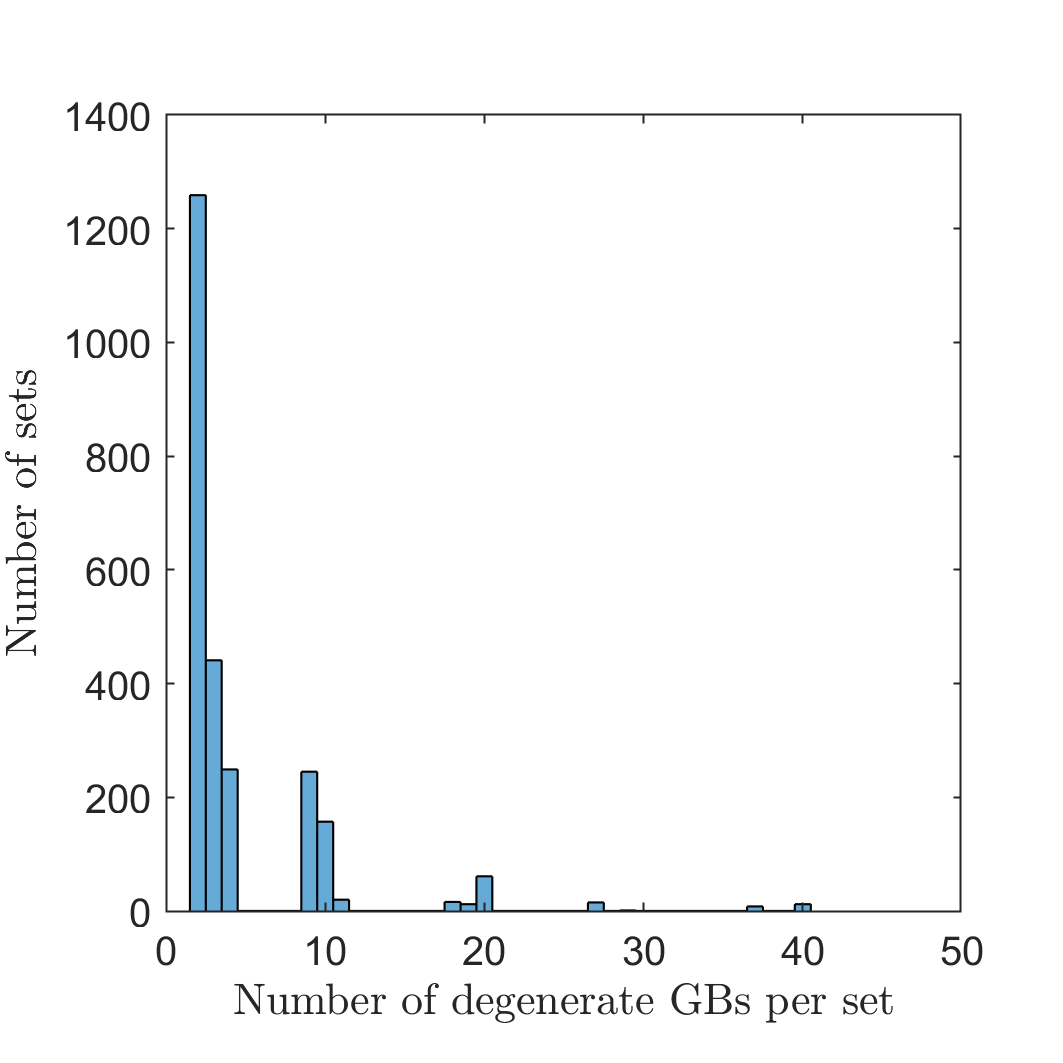
\includegraphics[scale=1]{kim-interp-degeneracy-sets.png}
		\caption{Histogram of number of sets vs. number of degenerate \glspl{gb} per set for the Fe simulation dataset \cite{kimPhasefieldModeling3D2014}. Most sets have a degeneracy of fewer than 5.}
		\label{fig:kim-interp-degeneracy-sets}
	\end{figure}
	
	\begin{figure}
		\centering
		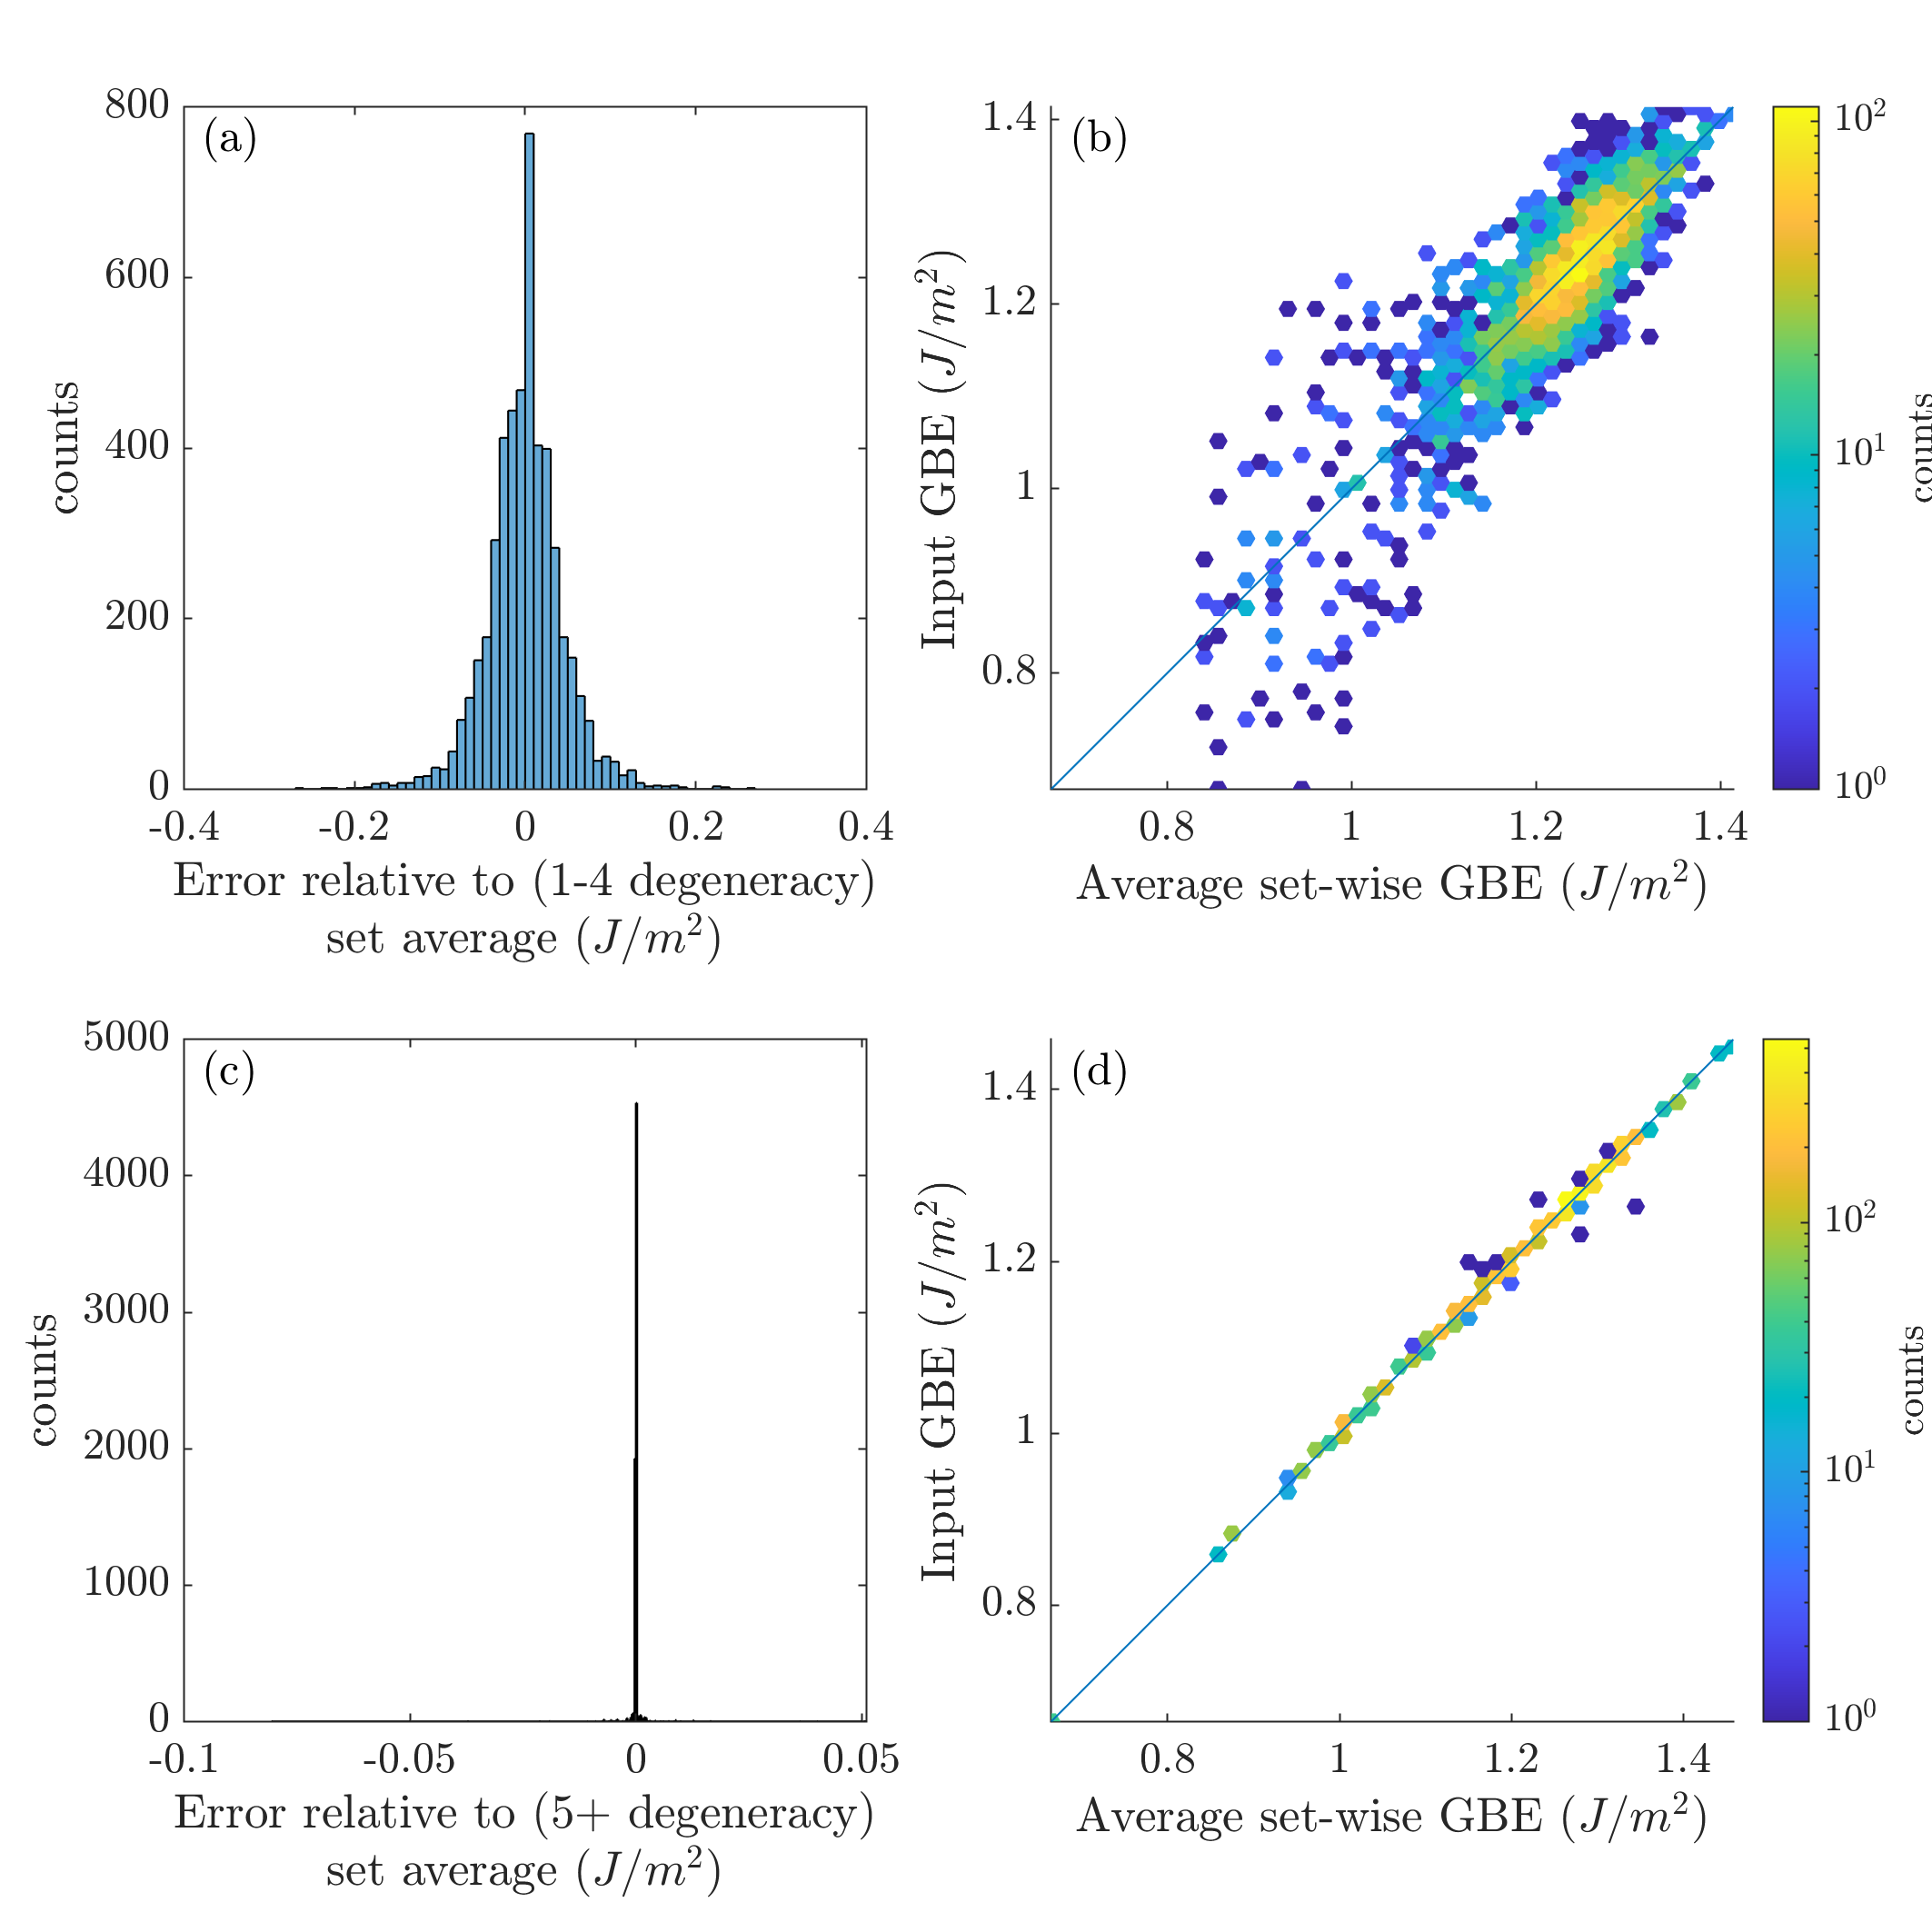
\includegraphics[scale=1]{kim-interp-degeneracy-results.png}
		\caption{Degenerate \glspl{gb} sets are split into those with a degeneracy of fewer than 5 and greater than or equal to 5 and plotted as ( (a) and (c), respectively) error histograms and ( (b) and (d), respectively) hexagonally-binned parity plots. Large degenerate sets tend to have very low error, whereas small degenerate sets tend to have higher error. In other words, \glspl{gb} that are more likely to be repeated many times based on the sampling scheme in \cite{kimPhasefieldModeling3D2014} tend to give similar results, whereas \glspl{gb} that are less likely to be repeated often have larger variability in the simulation output. We do not know if this has physical meaning or is an artifact of the simulation setup.}
		\label{fig:kim-interp-degeneracy-results}
	\end{figure}
	
	% \subsection{Uncertainty Quantification and the Posterior Distribution of \glsentrytitlecase{gprm}{long} }
	% The use of \gls{gpr} in the \gls{gprm} model facilitates uncertainty quantification which we discuss in more detail. We find that use of \cref{eq:gprmix-sigma} on two models with differing amounts of data leads to a model with typically higher uncertainty for low \glspl{gbe} than high \glspl{gbe} (\cref{fig:kim-interp-posterior}a). By observing the \glspl{nn} relative to an arc $\overline{AB}$, we find that there is a large scatter of \glspl{gbe} for \glspl{gb} that are within a radius of $\sim$\SI{6}{\degree} (\cref{fig:kim-interp-posterior}b). By sampling from the posterior distribution, we find that 
	
	% Uncertainty results, as well as posterior samples of the \gls{gprm} distribution of models are shown in \cref{fig:kim-interp-posterior}.
	
	% \begin{figure}
	%     \centering
	%     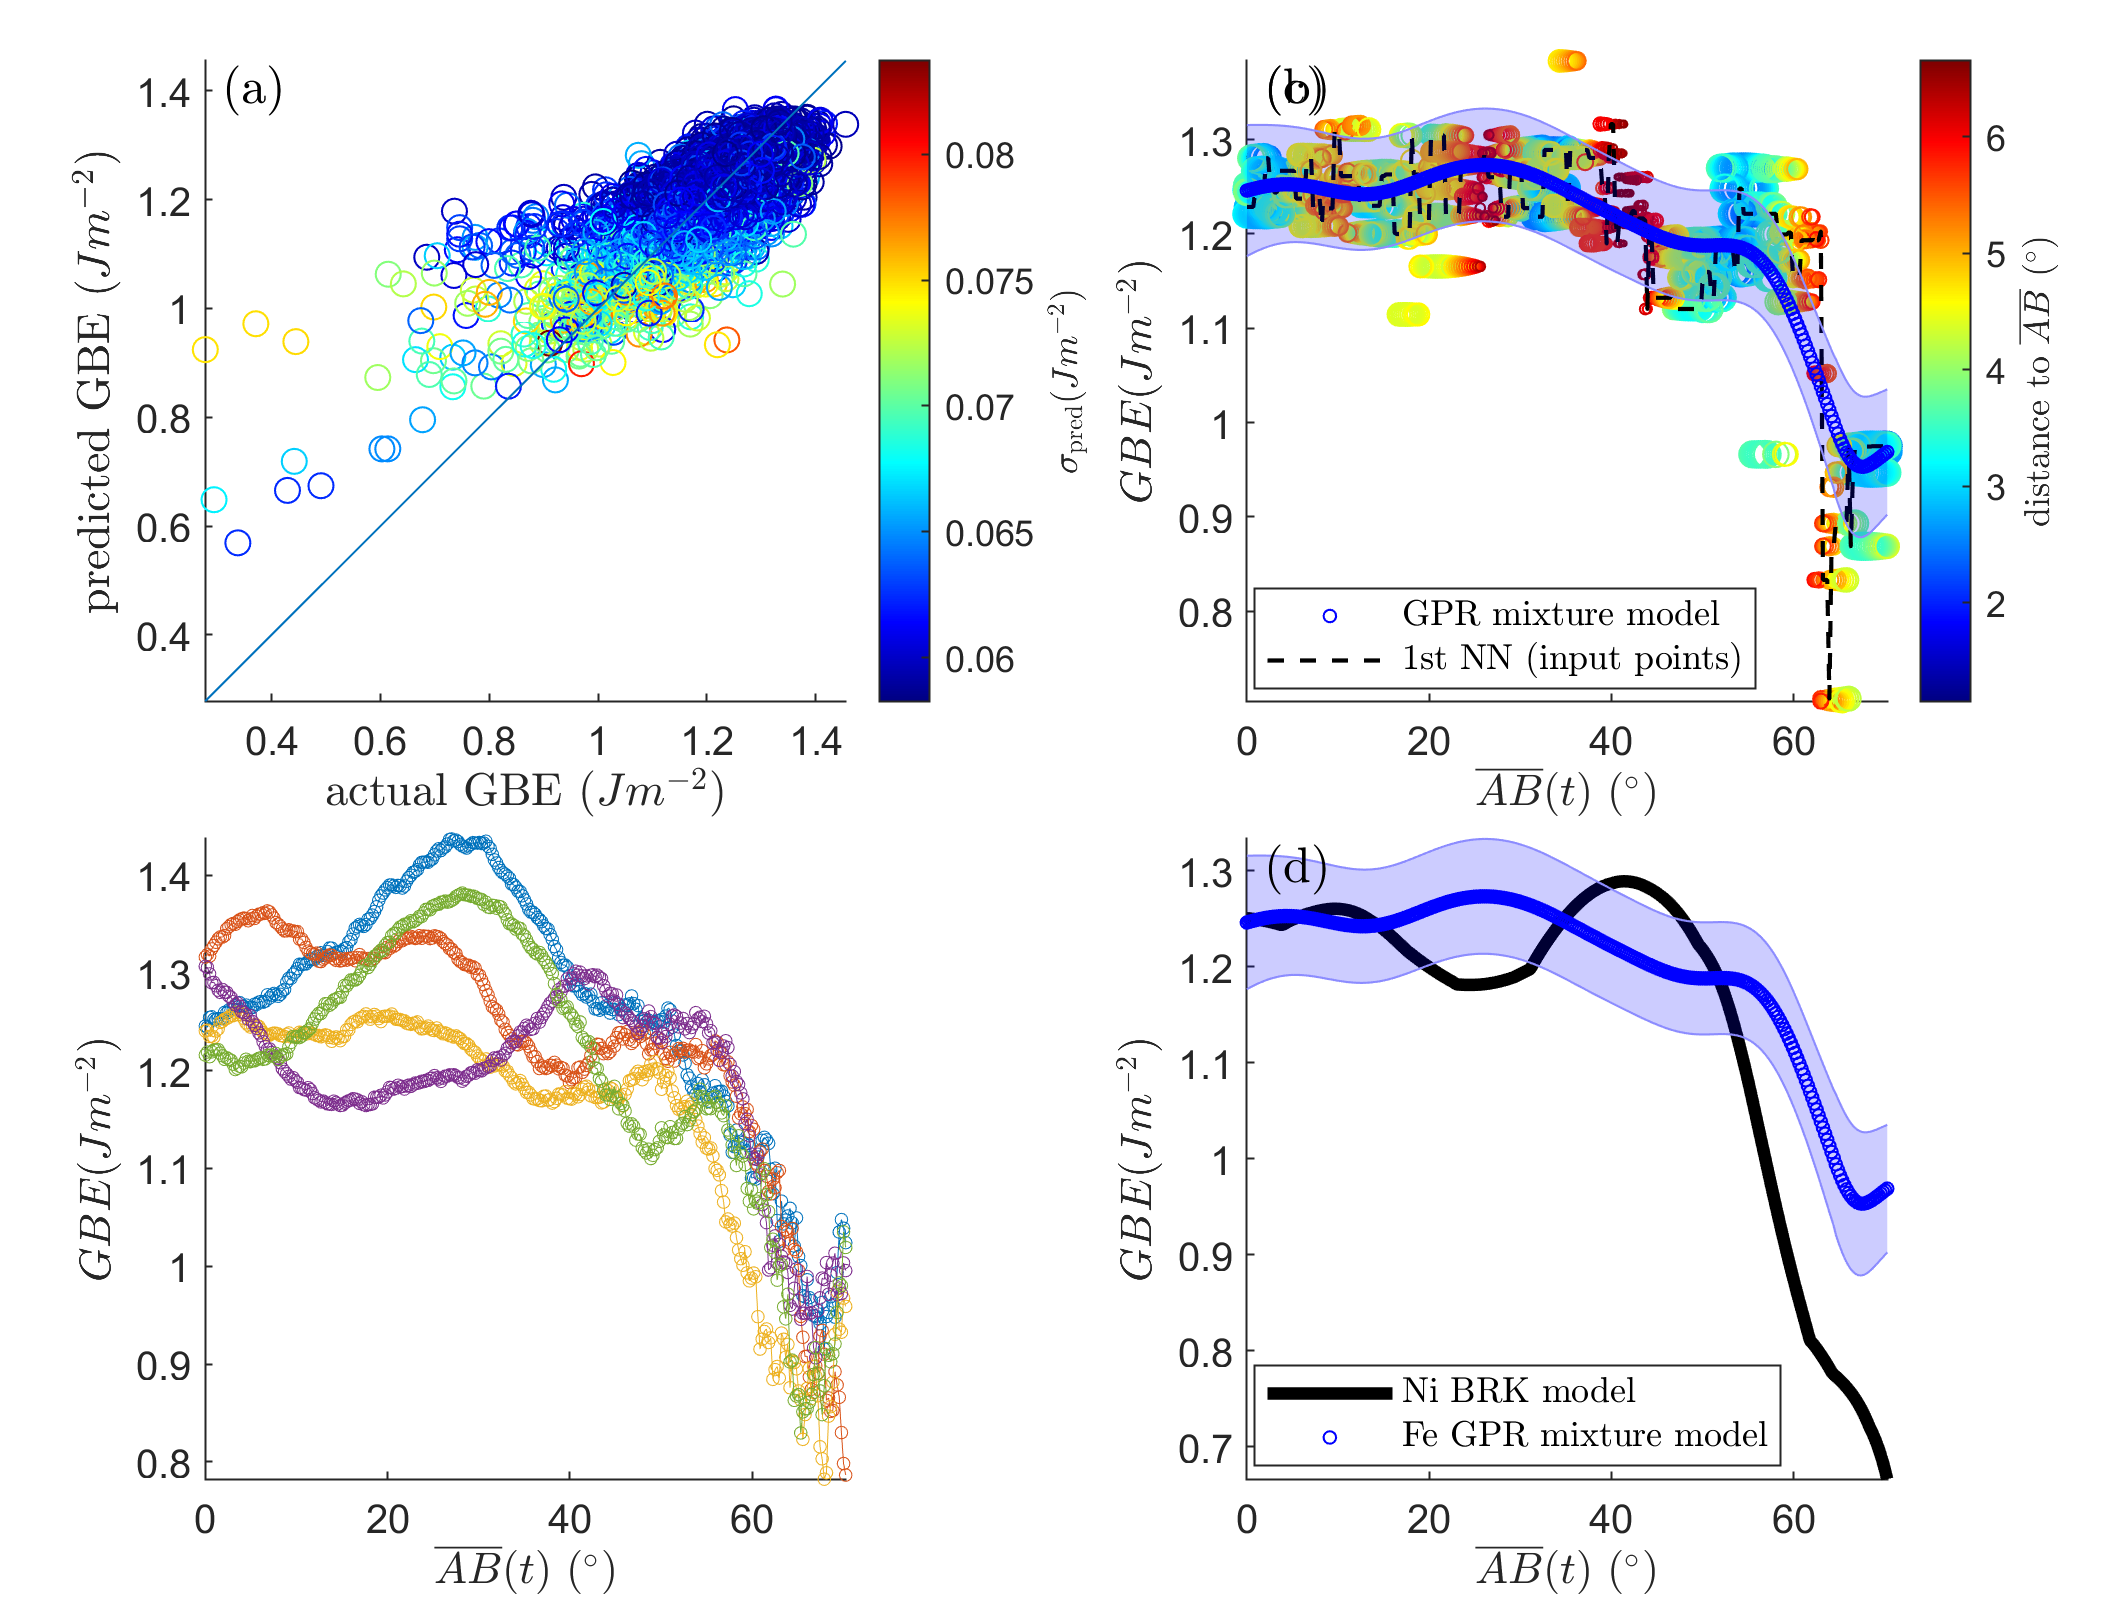
\includegraphics[scale=1]{figures/kim-interp-posterior.png}
	%     \caption{Interpolation results for a large Fe simulation database \cite{kimPhasefieldModeling3D2014} using \num{46883} \inpt{} \glspl{gb} and \num{11721} \outpt{} \glspl{gb} in an 80\%/20\% split and a \gls{gpr} mixture model to better approximate low \glspl{gbe}. (a) Parity plot colored by uncertainty standard deviation. (b) Prediction (black) and uncertainty standard deviation (grey band) of \gls{gpr} mixture model as a function of distance along a 1D arc ($\overline{AB}$) between two \glspl{vfzgbo} ($A$ and $B$). The first \inpt{} \gls{nn} is shown as a black, dashed line. The \inpt{} point \glspl{knn} ($k\in[1,2,3,4,5,6]$) relative to $\overline{AB}$ are colored and sized according to the distance to $\overline{AB}$ (\inpt{} points far from the line are small, dark red circles and \inpt{} points close to the line are large, dark blue circles). In other words, this shows the data in a small region of influence around $\overline{AB}$ that contributed to the model predictions where close data is emphasized (larger) than far-away data (smaller). (c)
	%     Five models sampled from the posterior distribution of the \gls{gpr} mixture model. (d) Fe \gls{gpr} mixture model results and uncertainty standard deviation (grey band) overlaid with the Ni \gls{brk} model along the arc $\overline{AB}$. Coordinates for $A$ and $B$ are given in \cref{tab:tunnel-AB2} of the main paper and 300 equally spaced points are plotted for (b), (c), and (d).}
	%     \label{fig:kim-interp-posterior}
	% \end{figure}

\bibliographystyle{elsarticle-num-names}
\bibliography{5dof-gb-energy.bib}

\end{document}